\documentclass[10pt,a4paper]{article}
\usepackage[utf8]{inputenc}
\usepackage[spanish]{babel}
\usepackage{amsmath, amsbsy, amssymb, amsthm, amsfonts}
\usepackage{graphicx}
\usepackage{multicol, multirow, array}
\usepackage{titling}
\usepackage{titlesec}
\usepackage{bm}
\usepackage{afterpage}
\usepackage{float}
\usepackage{epstopdf}
\usepackage{longtable}
\usepackage{xcolor}
\usepackage{epigraph} 
\setlength\epigraphwidth{1.5\textwidth}
\usepackage{subfigure}
\usepackage{anyfontsize}
\usepackage{listings}
\renewcommand{\lstlistingname}{Programa}% Listing -> Programa
\renewcommand{\lstlistlistingname}{List of \lstlistingname s}
\usepackage[left=2cm,right=2cm,top=2cm,bottom=2cm]{geometry}
\usepackage[colorlinks=true,
            linkcolor=blue,
            citecolor=blue,
            urlcolor=blue]{hyperref}
 %%%%%%%%%%%%%%%%%%%%%%%%%%%%%%%%%%%%%%%%%%%%%%%%%%%%%%%%%%%%%%%%%%%%%%%%%%%%%%%% 
%%% ~ Arduino Language - Arduino IDE Colors ~                                  %%%
%%%                                                                            %%%
%%% Kyle Rocha-Brownell | 10/2/2017 | No Licence                               %%%
%%% -------------------------------------------------------------------------- %%%
%%%                                                                            %%%
%%% Place this file in your working directory (next to the latex file you're   %%%
%%% working on).  To add it to your project, place:                            %%%
%%%     %%%%%%%%%%%%%%%%%%%%%%%%%%%%%%%%%%%%%%%%%%%%%%%%%%%%%%%%%%%%%%%%%%%%%%%%%%%%%%%% 
%%% ~ Arduino Language - Arduino IDE Colors ~                                  %%%
%%%                                                                            %%%
%%% Kyle Rocha-Brownell | 10/2/2017 | No Licence                               %%%
%%% -------------------------------------------------------------------------- %%%
%%%                                                                            %%%
%%% Place this file in your working directory (next to the latex file you're   %%%
%%% working on).  To add it to your project, place:                            %%%
%%%     %%%%%%%%%%%%%%%%%%%%%%%%%%%%%%%%%%%%%%%%%%%%%%%%%%%%%%%%%%%%%%%%%%%%%%%%%%%%%%%% 
%%% ~ Arduino Language - Arduino IDE Colors ~                                  %%%
%%%                                                                            %%%
%%% Kyle Rocha-Brownell | 10/2/2017 | No Licence                               %%%
%%% -------------------------------------------------------------------------- %%%
%%%                                                                            %%%
%%% Place this file in your working directory (next to the latex file you're   %%%
%%% working on).  To add it to your project, place:                            %%%
%%%    \input{arduinoLanguage.tex}                                             %%%
%%% somewhere before \begin{document} in your latex file.                      %%%
%%%                                                                            %%%
%%% In your document, place your arduino code between:                         %%%
%%%   \begin{lstlisting}[language=Arduino]                                     %%%
%%% and:                                                                       %%%
%%%   \end{lstlisting}                                                         %%%
%%%                                                                            %%%
%%% Or create your own style to add non-built-in functions and variables.      %%%
%%%                                                                            %%%
 %%%%%%%%%%%%%%%%%%%%%%%%%%%%%%%%%%%%%%%%%%%%%%%%%%%%%%%%%%%%%%%%%%%%%%%%%%%%%%%% 

\usepackage{color}
\usepackage{listings}    
\usepackage{courier}

%%% Define Custom IDE Colors %%%
\definecolor{arduinoGreen}    {rgb} {0.17, 0.43, 0.01}
\definecolor{arduinoGrey}     {rgb} {0.47, 0.47, 0.33}
\definecolor{arduinoOrange}   {rgb} {0.8 , 0.4 , 0   }
\definecolor{arduinoBlue}     {rgb} {0.01, 0.61, 0.98}
\definecolor{arduinoDarkBlue} {rgb} {0.0 , 0.2 , 0.5 }

%%% Define Arduino Language %%%
\lstdefinelanguage{Arduino}{
  language=C++, % begin with default C++ settings 
%
%
  %%% Keyword Color Group 1 %%%  (called KEYWORD3 by arduino)
  keywordstyle=\color{arduinoGreen},   
  deletekeywords={  % remove all arduino keywords that might be in c++
                break, case, override, final, continue, default, do, else, for, 
                if, return, goto, switch, throw, try, while, setup, loop, export, 
                not, or, and, xor, include, define, elif, else, error, if, ifdef, 
                ifndef, pragma, warning,
                HIGH, LOW, INPUT, INPUT_PULLUP, OUTPUT, DEC, BIN, HEX, OCT, PI, 
                HALF_PI, TWO_PI, LSBFIRST, MSBFIRST, CHANGE, FALLING, RISING, 
                DEFAULT, EXTERNAL, INTERNAL, INTERNAL1V1, INTERNAL2V56, LED_BUILTIN, 
                LED_BUILTIN_RX, LED_BUILTIN_TX, DIGITAL_MESSAGE, FIRMATA_STRING, 
                ANALOG_MESSAGE, REPORT_DIGITAL, REPORT_ANALOG, SET_PIN_MODE, 
                SYSTEM_RESET, SYSEX_START, auto, int8_t, int16_t, int32_t, int64_t, 
                uint8_t, uint16_t, uint32_t, uint64_t, char16_t, char32_t, operator, 
                enum, delete, bool, boolean, byte, char, const, false, float, double, 
                null, NULL, int, long, new, private, protected, public, short, 
                signed, static, volatile, String, void, true, unsigned, word, array, 
                sizeof, dynamic_cast, typedef, const_cast, struct, static_cast, union, 
                friend, extern, class, reinterpret_cast, register, explicit, inline, 
                _Bool, complex, _Complex, _Imaginary, atomic_bool, atomic_char, 
                atomic_schar, atomic_uchar, atomic_short, atomic_ushort, atomic_int, 
                atomic_uint, atomic_long, atomic_ulong, atomic_llong, atomic_ullong, 
                virtual, PROGMEM,
                Serial, Serial1, Serial2, Serial3, SerialUSB, Keyboard, Mouse,
                abs, acos, asin, atan, atan2, ceil, constrain, cos, degrees, exp, 
                floor, log, map, max, min, radians, random, randomSeed, round, sin, 
                sq, sqrt, tan, pow, bitRead, bitWrite, bitSet, bitClear, bit, 
                highByte, lowByte, analogReference, analogRead, 
                analogReadResolution, analogWrite, analogWriteResolution, 
                attachInterrupt, detachInterrupt, digitalPinToInterrupt, delay, 
                delayMicroseconds, digitalWrite, digitalRead, interrupts, millis, 
                micros, noInterrupts, noTone, pinMode, pulseIn, pulseInLong, shiftIn, 
                shiftOut, tone, yield, Stream, begin, end, peek, read, print, 
                println, available, availableForWrite, flush, setTimeout, find, 
                findUntil, parseInt, parseFloat, readBytes, readBytesUntil, readString, 
                readStringUntil, trim, toUpperCase, toLowerCase, charAt, compareTo, 
                concat, endsWith, startsWith, equals, equalsIgnoreCase, getBytes, 
                indexOf, lastIndexOf, length, replace, setCharAt, substring, 
                toCharArray, toInt, press, release, releaseAll, accept, click, move, 
                isPressed, isAlphaNumeric, isAlpha, isAscii, isWhitespace, isControl, 
                isDigit, isGraph, isLowerCase, isPrintable, isPunct, isSpace, 
                isUpperCase, isHexadecimalDigit, 
                }, 
  morekeywords={   % add arduino structures to group 1
                break, case, override, final, continue, default, do, else, for, 
                if, return, goto, switch, throw, try, while, setup, loop, export, 
                not, or, and, xor, include, define, elif, else, error, if, ifdef, 
                ifndef, pragma, warning,
                }, 
% 
%
  %%% Keyword Color Group 2 %%%  (called LITERAL1 by arduino)
  keywordstyle=[2]\color{arduinoBlue},   
  keywords=[2]{   % add variables and dataTypes as 2nd group  
                HIGH, LOW, INPUT, INPUT_PULLUP, OUTPUT, DEC, BIN, HEX, OCT, PI, 
                HALF_PI, TWO_PI, LSBFIRST, MSBFIRST, CHANGE, FALLING, RISING, 
                DEFAULT, EXTERNAL, INTERNAL, INTERNAL1V1, INTERNAL2V56, LED_BUILTIN, 
                LED_BUILTIN_RX, LED_BUILTIN_TX, DIGITAL_MESSAGE, FIRMATA_STRING, 
                ANALOG_MESSAGE, REPORT_DIGITAL, REPORT_ANALOG, SET_PIN_MODE, 
                SYSTEM_RESET, SYSEX_START, auto, int8_t, int16_t, int32_t, int64_t, 
                uint8_t, uint16_t, uint32_t, uint64_t, char16_t, char32_t, operator, 
                enum, delete, bool, boolean, byte, char, const, false, float, double, 
                null, NULL, int, long, new, private, protected, public, short, 
                signed, static, volatile, String, void, true, unsigned, word, array, 
                sizeof, dynamic_cast, typedef, const_cast, struct, static_cast, union, 
                friend, extern, class, reinterpret_cast, register, explicit, inline, 
                _Bool, complex, _Complex, _Imaginary, atomic_bool, atomic_char, 
                atomic_schar, atomic_uchar, atomic_short, atomic_ushort, atomic_int, 
                atomic_uint, atomic_long, atomic_ulong, atomic_llong, atomic_ullong, 
                virtual, PROGMEM,
                },  
% 
%
  %%% Keyword Color Group 3 %%%  (called KEYWORD1 by arduino)
  keywordstyle=[3]\bfseries\color{arduinoOrange},
  keywords=[3]{  % add built-in functions as a 3rd group
                Serial, Serial1, Serial2, Serial3, SerialUSB, Keyboard, Mouse, EEPROM,
                TimerOne},      
%
%
  %%% Keyword Color Group 4 %%%  (called KEYWORD2 by arduino)
  keywordstyle=[4]\color{arduinoOrange},
  keywords=[4]{  % add more built-in functions as a 4th group
                abs, acos, asin, atan, atan2, ceil, constrain, cos, degrees, exp, 
                floor, log, map, max, min, radians, random, randomSeed, round, sin, 
                sq, sqrt, tan, pow, bitRead, bitWrite, bitSet, bitClear, bit, 
                highByte, lowByte, analogReference, analogRead, 
                analogReadResolution, analogWrite, analogWriteResolution, 
                attachInterrupt, detachInterrupt, digitalPinToInterrupt, delay, 
                delayMicroseconds, digitalWrite, digitalRead, interrupts, millis, 
                micros, noInterrupts, noTone, pinMode, pulseIn, pulseInLong, shiftIn, 
                shiftOut, tone, yield, Stream, begin, end, peek, read, print, 
                println, available, availableForWrite, flush, setTimeout, find, 
                findUntil, parseInt, parseFloat, readBytes, readBytesUntil, readString, 
                readStringUntil, trim, toUpperCase, toLowerCase, charAt, compareTo, 
                concat, endsWith, startsWith, equals, equalsIgnoreCase, getBytes, 
                indexOf, lastIndexOf, length, replace, setCharAt, substring, 
                toCharArray, toInt, press, release, releaseAll, accept, click, move, 
                isPressed, isAlphaNumeric, isAlpha, isAscii, isWhitespace, isControl, 
                isDigit, isGraph, isLowerCase, isPrintable, isPunct, isSpace, 
                isUpperCase, isHexadecimalDigit, 
                },      
%
%
  %%% Set Other Colors %%%
  stringstyle=\color{arduinoDarkBlue},    
  commentstyle=\color{arduinoGrey},    
%          
%   
  %%%% Line Numbering %%%%
   numbers=left,                    
  numbersep=5pt,                   
  numberstyle=\color{arduinoGrey},    
  %stepnumber=2,                      % show every 2 line numbers
%
%
  %%%% Code Box Style %%%%
  breaklines=true,                    % wordwrapping
  tabsize=2,
  frame=shadowbox,
  rulesepcolor=\color{arduinoBlue},         
  basicstyle=\ttfamily  
}                                             %%%
%%% somewhere before \begin{document} in your latex file.                      %%%
%%%                                                                            %%%
%%% In your document, place your arduino code between:                         %%%
%%%   \begin{lstlisting}[language=Arduino]                                     %%%
%%% and:                                                                       %%%
%%%   \end{lstlisting}                                                         %%%
%%%                                                                            %%%
%%% Or create your own style to add non-built-in functions and variables.      %%%
%%%                                                                            %%%
 %%%%%%%%%%%%%%%%%%%%%%%%%%%%%%%%%%%%%%%%%%%%%%%%%%%%%%%%%%%%%%%%%%%%%%%%%%%%%%%% 

\usepackage{color}
\usepackage{listings}    
\usepackage{courier}

%%% Define Custom IDE Colors %%%
\definecolor{arduinoGreen}    {rgb} {0.17, 0.43, 0.01}
\definecolor{arduinoGrey}     {rgb} {0.47, 0.47, 0.33}
\definecolor{arduinoOrange}   {rgb} {0.8 , 0.4 , 0   }
\definecolor{arduinoBlue}     {rgb} {0.01, 0.61, 0.98}
\definecolor{arduinoDarkBlue} {rgb} {0.0 , 0.2 , 0.5 }

%%% Define Arduino Language %%%
\lstdefinelanguage{Arduino}{
  language=C++, % begin with default C++ settings 
%
%
  %%% Keyword Color Group 1 %%%  (called KEYWORD3 by arduino)
  keywordstyle=\color{arduinoGreen},   
  deletekeywords={  % remove all arduino keywords that might be in c++
                break, case, override, final, continue, default, do, else, for, 
                if, return, goto, switch, throw, try, while, setup, loop, export, 
                not, or, and, xor, include, define, elif, else, error, if, ifdef, 
                ifndef, pragma, warning,
                HIGH, LOW, INPUT, INPUT_PULLUP, OUTPUT, DEC, BIN, HEX, OCT, PI, 
                HALF_PI, TWO_PI, LSBFIRST, MSBFIRST, CHANGE, FALLING, RISING, 
                DEFAULT, EXTERNAL, INTERNAL, INTERNAL1V1, INTERNAL2V56, LED_BUILTIN, 
                LED_BUILTIN_RX, LED_BUILTIN_TX, DIGITAL_MESSAGE, FIRMATA_STRING, 
                ANALOG_MESSAGE, REPORT_DIGITAL, REPORT_ANALOG, SET_PIN_MODE, 
                SYSTEM_RESET, SYSEX_START, auto, int8_t, int16_t, int32_t, int64_t, 
                uint8_t, uint16_t, uint32_t, uint64_t, char16_t, char32_t, operator, 
                enum, delete, bool, boolean, byte, char, const, false, float, double, 
                null, NULL, int, long, new, private, protected, public, short, 
                signed, static, volatile, String, void, true, unsigned, word, array, 
                sizeof, dynamic_cast, typedef, const_cast, struct, static_cast, union, 
                friend, extern, class, reinterpret_cast, register, explicit, inline, 
                _Bool, complex, _Complex, _Imaginary, atomic_bool, atomic_char, 
                atomic_schar, atomic_uchar, atomic_short, atomic_ushort, atomic_int, 
                atomic_uint, atomic_long, atomic_ulong, atomic_llong, atomic_ullong, 
                virtual, PROGMEM,
                Serial, Serial1, Serial2, Serial3, SerialUSB, Keyboard, Mouse,
                abs, acos, asin, atan, atan2, ceil, constrain, cos, degrees, exp, 
                floor, log, map, max, min, radians, random, randomSeed, round, sin, 
                sq, sqrt, tan, pow, bitRead, bitWrite, bitSet, bitClear, bit, 
                highByte, lowByte, analogReference, analogRead, 
                analogReadResolution, analogWrite, analogWriteResolution, 
                attachInterrupt, detachInterrupt, digitalPinToInterrupt, delay, 
                delayMicroseconds, digitalWrite, digitalRead, interrupts, millis, 
                micros, noInterrupts, noTone, pinMode, pulseIn, pulseInLong, shiftIn, 
                shiftOut, tone, yield, Stream, begin, end, peek, read, print, 
                println, available, availableForWrite, flush, setTimeout, find, 
                findUntil, parseInt, parseFloat, readBytes, readBytesUntil, readString, 
                readStringUntil, trim, toUpperCase, toLowerCase, charAt, compareTo, 
                concat, endsWith, startsWith, equals, equalsIgnoreCase, getBytes, 
                indexOf, lastIndexOf, length, replace, setCharAt, substring, 
                toCharArray, toInt, press, release, releaseAll, accept, click, move, 
                isPressed, isAlphaNumeric, isAlpha, isAscii, isWhitespace, isControl, 
                isDigit, isGraph, isLowerCase, isPrintable, isPunct, isSpace, 
                isUpperCase, isHexadecimalDigit, 
                }, 
  morekeywords={   % add arduino structures to group 1
                break, case, override, final, continue, default, do, else, for, 
                if, return, goto, switch, throw, try, while, setup, loop, export, 
                not, or, and, xor, include, define, elif, else, error, if, ifdef, 
                ifndef, pragma, warning,
                }, 
% 
%
  %%% Keyword Color Group 2 %%%  (called LITERAL1 by arduino)
  keywordstyle=[2]\color{arduinoBlue},   
  keywords=[2]{   % add variables and dataTypes as 2nd group  
                HIGH, LOW, INPUT, INPUT_PULLUP, OUTPUT, DEC, BIN, HEX, OCT, PI, 
                HALF_PI, TWO_PI, LSBFIRST, MSBFIRST, CHANGE, FALLING, RISING, 
                DEFAULT, EXTERNAL, INTERNAL, INTERNAL1V1, INTERNAL2V56, LED_BUILTIN, 
                LED_BUILTIN_RX, LED_BUILTIN_TX, DIGITAL_MESSAGE, FIRMATA_STRING, 
                ANALOG_MESSAGE, REPORT_DIGITAL, REPORT_ANALOG, SET_PIN_MODE, 
                SYSTEM_RESET, SYSEX_START, auto, int8_t, int16_t, int32_t, int64_t, 
                uint8_t, uint16_t, uint32_t, uint64_t, char16_t, char32_t, operator, 
                enum, delete, bool, boolean, byte, char, const, false, float, double, 
                null, NULL, int, long, new, private, protected, public, short, 
                signed, static, volatile, String, void, true, unsigned, word, array, 
                sizeof, dynamic_cast, typedef, const_cast, struct, static_cast, union, 
                friend, extern, class, reinterpret_cast, register, explicit, inline, 
                _Bool, complex, _Complex, _Imaginary, atomic_bool, atomic_char, 
                atomic_schar, atomic_uchar, atomic_short, atomic_ushort, atomic_int, 
                atomic_uint, atomic_long, atomic_ulong, atomic_llong, atomic_ullong, 
                virtual, PROGMEM,
                },  
% 
%
  %%% Keyword Color Group 3 %%%  (called KEYWORD1 by arduino)
  keywordstyle=[3]\bfseries\color{arduinoOrange},
  keywords=[3]{  % add built-in functions as a 3rd group
                Serial, Serial1, Serial2, Serial3, SerialUSB, Keyboard, Mouse, EEPROM,
                TimerOne},      
%
%
  %%% Keyword Color Group 4 %%%  (called KEYWORD2 by arduino)
  keywordstyle=[4]\color{arduinoOrange},
  keywords=[4]{  % add more built-in functions as a 4th group
                abs, acos, asin, atan, atan2, ceil, constrain, cos, degrees, exp, 
                floor, log, map, max, min, radians, random, randomSeed, round, sin, 
                sq, sqrt, tan, pow, bitRead, bitWrite, bitSet, bitClear, bit, 
                highByte, lowByte, analogReference, analogRead, 
                analogReadResolution, analogWrite, analogWriteResolution, 
                attachInterrupt, detachInterrupt, digitalPinToInterrupt, delay, 
                delayMicroseconds, digitalWrite, digitalRead, interrupts, millis, 
                micros, noInterrupts, noTone, pinMode, pulseIn, pulseInLong, shiftIn, 
                shiftOut, tone, yield, Stream, begin, end, peek, read, print, 
                println, available, availableForWrite, flush, setTimeout, find, 
                findUntil, parseInt, parseFloat, readBytes, readBytesUntil, readString, 
                readStringUntil, trim, toUpperCase, toLowerCase, charAt, compareTo, 
                concat, endsWith, startsWith, equals, equalsIgnoreCase, getBytes, 
                indexOf, lastIndexOf, length, replace, setCharAt, substring, 
                toCharArray, toInt, press, release, releaseAll, accept, click, move, 
                isPressed, isAlphaNumeric, isAlpha, isAscii, isWhitespace, isControl, 
                isDigit, isGraph, isLowerCase, isPrintable, isPunct, isSpace, 
                isUpperCase, isHexadecimalDigit, 
                },      
%
%
  %%% Set Other Colors %%%
  stringstyle=\color{arduinoDarkBlue},    
  commentstyle=\color{arduinoGrey},    
%          
%   
  %%%% Line Numbering %%%%
   numbers=left,                    
  numbersep=5pt,                   
  numberstyle=\color{arduinoGrey},    
  %stepnumber=2,                      % show every 2 line numbers
%
%
  %%%% Code Box Style %%%%
  breaklines=true,                    % wordwrapping
  tabsize=2,
  frame=shadowbox,
  rulesepcolor=\color{arduinoBlue},         
  basicstyle=\ttfamily  
}                                             %%%
%%% somewhere before \begin{document} in your latex file.                      %%%
%%%                                                                            %%%
%%% In your document, place your arduino code between:                         %%%
%%%   \begin{lstlisting}[language=Arduino]                                     %%%
%%% and:                                                                       %%%
%%%   \end{lstlisting}                                                         %%%
%%%                                                                            %%%
%%% Or create your own style to add non-built-in functions and variables.      %%%
%%%                                                                            %%%
 %%%%%%%%%%%%%%%%%%%%%%%%%%%%%%%%%%%%%%%%%%%%%%%%%%%%%%%%%%%%%%%%%%%%%%%%%%%%%%%% 

\usepackage{color}
\usepackage{listings}    
\usepackage{courier}

%%% Define Custom IDE Colors %%%
\definecolor{arduinoGreen}    {rgb} {0.17, 0.43, 0.01}
\definecolor{arduinoGrey}     {rgb} {0.47, 0.47, 0.33}
\definecolor{arduinoOrange}   {rgb} {0.8 , 0.4 , 0   }
\definecolor{arduinoBlue}     {rgb} {0.01, 0.61, 0.98}
\definecolor{arduinoDarkBlue} {rgb} {0.0 , 0.2 , 0.5 }

%%% Define Arduino Language %%%
\lstdefinelanguage{Arduino}{
  language=C++, % begin with default C++ settings 
%
%
  %%% Keyword Color Group 1 %%%  (called KEYWORD3 by arduino)
  keywordstyle=\color{arduinoGreen},   
  deletekeywords={  % remove all arduino keywords that might be in c++
                break, case, override, final, continue, default, do, else, for, 
                if, return, goto, switch, throw, try, while, setup, loop, export, 
                not, or, and, xor, include, define, elif, else, error, if, ifdef, 
                ifndef, pragma, warning,
                HIGH, LOW, INPUT, INPUT_PULLUP, OUTPUT, DEC, BIN, HEX, OCT, PI, 
                HALF_PI, TWO_PI, LSBFIRST, MSBFIRST, CHANGE, FALLING, RISING, 
                DEFAULT, EXTERNAL, INTERNAL, INTERNAL1V1, INTERNAL2V56, LED_BUILTIN, 
                LED_BUILTIN_RX, LED_BUILTIN_TX, DIGITAL_MESSAGE, FIRMATA_STRING, 
                ANALOG_MESSAGE, REPORT_DIGITAL, REPORT_ANALOG, SET_PIN_MODE, 
                SYSTEM_RESET, SYSEX_START, auto, int8_t, int16_t, int32_t, int64_t, 
                uint8_t, uint16_t, uint32_t, uint64_t, char16_t, char32_t, operator, 
                enum, delete, bool, boolean, byte, char, const, false, float, double, 
                null, NULL, int, long, new, private, protected, public, short, 
                signed, static, volatile, String, void, true, unsigned, word, array, 
                sizeof, dynamic_cast, typedef, const_cast, struct, static_cast, union, 
                friend, extern, class, reinterpret_cast, register, explicit, inline, 
                _Bool, complex, _Complex, _Imaginary, atomic_bool, atomic_char, 
                atomic_schar, atomic_uchar, atomic_short, atomic_ushort, atomic_int, 
                atomic_uint, atomic_long, atomic_ulong, atomic_llong, atomic_ullong, 
                virtual, PROGMEM,
                Serial, Serial1, Serial2, Serial3, SerialUSB, Keyboard, Mouse,
                abs, acos, asin, atan, atan2, ceil, constrain, cos, degrees, exp, 
                floor, log, map, max, min, radians, random, randomSeed, round, sin, 
                sq, sqrt, tan, pow, bitRead, bitWrite, bitSet, bitClear, bit, 
                highByte, lowByte, analogReference, analogRead, 
                analogReadResolution, analogWrite, analogWriteResolution, 
                attachInterrupt, detachInterrupt, digitalPinToInterrupt, delay, 
                delayMicroseconds, digitalWrite, digitalRead, interrupts, millis, 
                micros, noInterrupts, noTone, pinMode, pulseIn, pulseInLong, shiftIn, 
                shiftOut, tone, yield, Stream, begin, end, peek, read, print, 
                println, available, availableForWrite, flush, setTimeout, find, 
                findUntil, parseInt, parseFloat, readBytes, readBytesUntil, readString, 
                readStringUntil, trim, toUpperCase, toLowerCase, charAt, compareTo, 
                concat, endsWith, startsWith, equals, equalsIgnoreCase, getBytes, 
                indexOf, lastIndexOf, length, replace, setCharAt, substring, 
                toCharArray, toInt, press, release, releaseAll, accept, click, move, 
                isPressed, isAlphaNumeric, isAlpha, isAscii, isWhitespace, isControl, 
                isDigit, isGraph, isLowerCase, isPrintable, isPunct, isSpace, 
                isUpperCase, isHexadecimalDigit, 
                }, 
  morekeywords={   % add arduino structures to group 1
                break, case, override, final, continue, default, do, else, for, 
                if, return, goto, switch, throw, try, while, setup, loop, export, 
                not, or, and, xor, include, define, elif, else, error, if, ifdef, 
                ifndef, pragma, warning,
                }, 
% 
%
  %%% Keyword Color Group 2 %%%  (called LITERAL1 by arduino)
  keywordstyle=[2]\color{arduinoBlue},   
  keywords=[2]{   % add variables and dataTypes as 2nd group  
                HIGH, LOW, INPUT, INPUT_PULLUP, OUTPUT, DEC, BIN, HEX, OCT, PI, 
                HALF_PI, TWO_PI, LSBFIRST, MSBFIRST, CHANGE, FALLING, RISING, 
                DEFAULT, EXTERNAL, INTERNAL, INTERNAL1V1, INTERNAL2V56, LED_BUILTIN, 
                LED_BUILTIN_RX, LED_BUILTIN_TX, DIGITAL_MESSAGE, FIRMATA_STRING, 
                ANALOG_MESSAGE, REPORT_DIGITAL, REPORT_ANALOG, SET_PIN_MODE, 
                SYSTEM_RESET, SYSEX_START, auto, int8_t, int16_t, int32_t, int64_t, 
                uint8_t, uint16_t, uint32_t, uint64_t, char16_t, char32_t, operator, 
                enum, delete, bool, boolean, byte, char, const, false, float, double, 
                null, NULL, int, long, new, private, protected, public, short, 
                signed, static, volatile, String, void, true, unsigned, word, array, 
                sizeof, dynamic_cast, typedef, const_cast, struct, static_cast, union, 
                friend, extern, class, reinterpret_cast, register, explicit, inline, 
                _Bool, complex, _Complex, _Imaginary, atomic_bool, atomic_char, 
                atomic_schar, atomic_uchar, atomic_short, atomic_ushort, atomic_int, 
                atomic_uint, atomic_long, atomic_ulong, atomic_llong, atomic_ullong, 
                virtual, PROGMEM,
                },  
% 
%
  %%% Keyword Color Group 3 %%%  (called KEYWORD1 by arduino)
  keywordstyle=[3]\bfseries\color{arduinoOrange},
  keywords=[3]{  % add built-in functions as a 3rd group
                Serial, Serial1, Serial2, Serial3, SerialUSB, Keyboard, Mouse, EEPROM,
                TimerOne},      
%
%
  %%% Keyword Color Group 4 %%%  (called KEYWORD2 by arduino)
  keywordstyle=[4]\color{arduinoOrange},
  keywords=[4]{  % add more built-in functions as a 4th group
                abs, acos, asin, atan, atan2, ceil, constrain, cos, degrees, exp, 
                floor, log, map, max, min, radians, random, randomSeed, round, sin, 
                sq, sqrt, tan, pow, bitRead, bitWrite, bitSet, bitClear, bit, 
                highByte, lowByte, analogReference, analogRead, 
                analogReadResolution, analogWrite, analogWriteResolution, 
                attachInterrupt, detachInterrupt, digitalPinToInterrupt, delay, 
                delayMicroseconds, digitalWrite, digitalRead, interrupts, millis, 
                micros, noInterrupts, noTone, pinMode, pulseIn, pulseInLong, shiftIn, 
                shiftOut, tone, yield, Stream, begin, end, peek, read, print, 
                println, available, availableForWrite, flush, setTimeout, find, 
                findUntil, parseInt, parseFloat, readBytes, readBytesUntil, readString, 
                readStringUntil, trim, toUpperCase, toLowerCase, charAt, compareTo, 
                concat, endsWith, startsWith, equals, equalsIgnoreCase, getBytes, 
                indexOf, lastIndexOf, length, replace, setCharAt, substring, 
                toCharArray, toInt, press, release, releaseAll, accept, click, move, 
                isPressed, isAlphaNumeric, isAlpha, isAscii, isWhitespace, isControl, 
                isDigit, isGraph, isLowerCase, isPrintable, isPunct, isSpace, 
                isUpperCase, isHexadecimalDigit, 
                },      
%
%
  %%% Set Other Colors %%%
  stringstyle=\color{arduinoDarkBlue},    
  commentstyle=\color{arduinoGrey},    
%          
%   
  %%%% Line Numbering %%%%
   numbers=left,                    
  numbersep=5pt,                   
  numberstyle=\color{arduinoGrey},    
  %stepnumber=2,                      % show every 2 line numbers
%
%
  %%%% Code Box Style %%%%
  breaklines=true,                    % wordwrapping
  tabsize=2,
  frame=shadowbox,
  rulesepcolor=\color{arduinoBlue},         
  basicstyle=\ttfamily  
}

\begin{document}
\author{Benavides Wilmer, Farinango Luis, Velasco Angel}
\title{UNIVERSIDAD TÉCNICA DEL NORTE \\
FICA-CIERCOM\\
SISTEMAS EMBEBIDOS\\
Análisis de Datos}
\maketitle
\section{Introducción}
Si se analiza una base de datos con algoritmos de clasificación ,en la mayoría de los casos  existirán valores redundantes que entorpecerán el rendimiento del algoritmo o modelo, así como métodos más efectivos de acuerdo a como se analice los datos antes de la aplicación de dichos algoritmos .Por estas razones existen métodos que indican cuan exacto es un algoritmo o que devuelven los porcentajes de variables que pueden ser consideradas despreciables .
\section{Marco Teórico}

\subsection{Matriz de Confusión}
Una Matriz de Confusión es un método de evaluación de un modelo de clasificación, es decir que ayuda a determinar que tan bien clasifica un algoritmo determinado. Para esto se debe contar con los datos presentados en el Cuadro~ \ref{tab:confusion}.
\begin{table}[H]
  	\centering
  	\caption{Matriz de confusión}
	\begin{tabular}{c  >{\centering\arraybackslash}m{2cm}|>{\centering\arraybackslash}m{3cm}|>{\centering\arraybackslash}m{3cm}|}
		\cline{3-4} 
 		&		& \multicolumn{2}{c|}{\textbf{Predicción}} \\
		\cline{3-4}  
 		&		& \textbf{Positivos} & \textbf{Negativos}\\
		\hline 
		\multicolumn{1}{|c|}{\multirow{2}{*}{\rotatebox{90}{\textbf{Observación}}}} 		& \textbf{Positivos} & Verdaderos Positivos (VP) & Falsos Negativos (FN)\\ 			[0.7cm]
		\cline{2-4} 
		\multicolumn{1}{|c|}{} 	& \textbf{Negativos} & Falsos Positivos (FP) & 				Verdaderos Negativos (VN) \\ [0.7cm]
		\hline 
	\end{tabular}%
	\label{tab:confusion}%
\end{table}
Donde se muestran los valores observados en las filas de cada tabla y los valores predichos por el algoritmos en las columnas de la misma para un clasificador binario. Las variables demostradas significan lo siguiente:\\
\paragraph{Verdaderos Positivos} donde obtenemos todos los valores positivos que el modelo pudo clasificar correctamente como positivos.
\paragraph{Falsos Negativos} donde obtenemos todos los valores positivos que el modelo clasifica incorrectamente como negativos.
\paragraph{Falsos Positivos} donde obtenemos todos los valores negativos que el modelo clasifica incorrectamente como positivos.
\paragraph{Verdaderos Negativos} donde obtenemos todos los valores negativos que el modelo pudo clasificar correctamente como negativos.

En un caso ideal obtendríamos
\begin{equation}
\begin{array}{cc}
1 & 0 \\ 
0 & 1
\end{array}
\end{equation}
pero, este caso se encuentra bastante alejado de la realidad, es decir que si llega a suceder estaríamos cometiendo un error en nuestro análisis.

\subsubsection{Especificidad (Especificity}
El porcentaje de elementos clasificados negativos en una base de datos de valores únicamente negativos, sigue la siguiente expresión:
\begin{equation}
Especificidad = \frac{VN}{Total Negativos}
\end{equation}


\subsubsection{Sensibilidad o exhaustividad (Sensitivity, Recall)}
Indica todos los valores que nuestro modelo clasificó como positivos en una base de datos de valores únicamente positivos, como se muestra en la Ecuación ~\ref{eq:tpr}
\begin{equation}
Sensibilidad = \frac{VP}{Total Positivos}
\label{eq:tpr}
\end{equation}

\subsubsection{Rendimiento de los algoritmos de clasificación}
Para obtener un valor cuantitativo que indique el rendimiento de los algoritmos de clasificación que se utilicen, se introducen la Formulas ~\ref{eq:acc} y \ref{eq:mr}. 
\subsubsection*{Exactitud (Accuracy)}
En general, es el porcentaje de datos que el algoritmo clasifica correctamente, se puede determinar de la siguiente manera:
\begin{equation}
Exactitud = \frac{VP+VN}{FP+FN}
\label{eq:acc}
\end{equation}

\subsubsection*{Tasa de error (Misclassification Rate)}
En general, es el porcentaje de datos que el algoritmo clasifica incorrectamente y se representa de la siguiente forma:
\begin{equation}
Error = \frac{FP+FN}{Total}
\label{eq:mr}
\end{equation}

\subsection{Curva ROC}
Una curva ROC proporciona una representación de la sensibilidad y especifidad para cada valor umbral, que es invariante mediante transformaciones monótonas a los datos de la variable de decisión y que permite comparar dos o más clasificadores en función de su función discriminante.\\
Un análisis ROC de sus siglas en ingles Receiver Operating Characteristics, es una metodología desarrollada para analizar un sistema de decisión. Este análisis se basa en las nociones de sensibilidad y especificidad.\\
Una curva ROC proporciona una representación de la sensibilidad generalmente ubicada en el eje de las “y” ,es decir se muestra los verdaderos positivos.
\begin{equation}
 \frac{(VP)}{ (VP)+  (FN)}
\end{equation}
Donde VP es el número de verdaderos positivos,FN es el número de falsos negativos.\\
La especificidad se ubica en el eje de las “x” y representa los falsos positivos .
\begin{equation}
 \frac{(FP)}{ (FP)+  (VN)}
\end{equation}
Donde FP es el número de falsos positivos,VN es el número de verdaderos negativos.\\
La curva basa sus dos valores sen función de cada valor umbral ,que es invariante mediante transformaciones monótonas a los datos de la variable de decisión y que permite comparar dos o más clasificadores en función de su función discriminante.
Además, en la curva ROC cada uno de los puntos representa un par de sensibilidad/especificidad correspondiente a un umbral de decisión particular.

\subsection{Medición AUC}
El área bajo la curva ROC (AUC) permite representar
en un único valor el rendimiento del clasificador. Esto
puede resultar útil para realizar comparativas entre
clasificadores.
\begin{equation}
AUC = \frac{1+TPR-FPR}{2}
\label{eq:acc}
\end{equation}
Donde TPR ES tasa positiva verdadera, FPR tasa de falsos positivos.\\

AUC representa el grado o medida de separabilidad.Indica cuánto modelo es capaz de distinguir entre clases.\\

La curva ROC se traza con TPR contra el FPR donde TPR está en el eje y y FPR está en el eje x.
\begin{figure}[H]
 \centering
 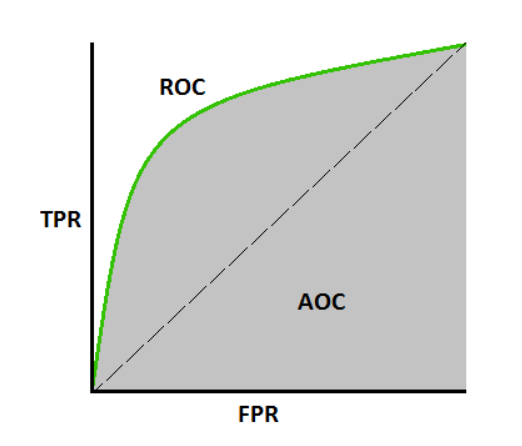
\includegraphics[scale=0.5]{AUCC.PNG}
 \caption{Curva ROC y AUC en funsión de TPR Y FPR}
 \end{figure}
Máximo AUC posible = 1
Un modelo excelente tiene AUC cerca del 1, lo que significa que tiene una buena medida de separabilidad. Un modelo pobre tiene AUC cerca del 0, lo que significa que tiene la peor medida de separabilidad.
\begin{figure}[H]
\centering
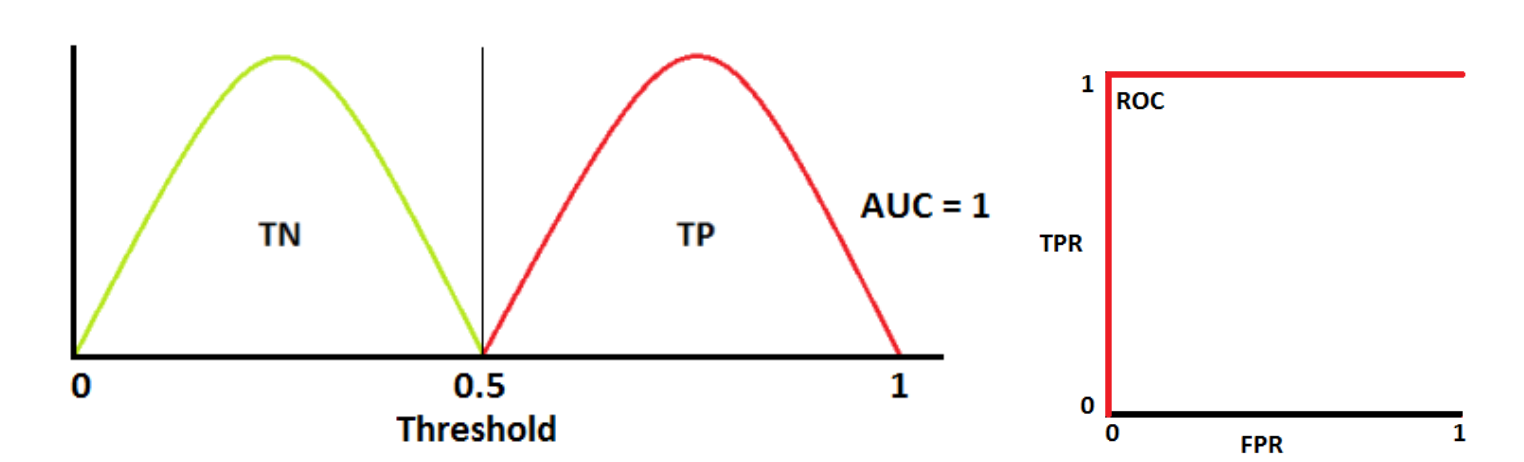
\includegraphics[scale=0.5]{AUC1.PNG}
\caption{AUC = 1}
\end{figure}
Cuando AUC es 0.7, significa que hay un 70 por ciento de posibilidades de que el modelo pueda distinguir entre clase positiva y clase negativa.
\begin{figure}[H]
\centering
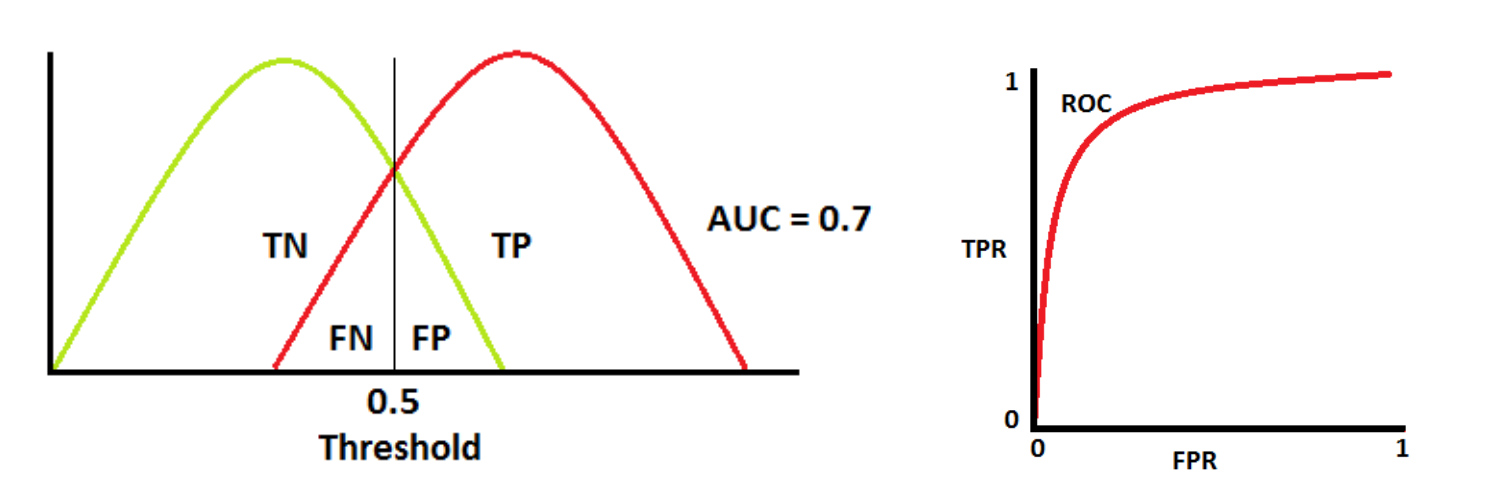
\includegraphics[scale=0.5]{AUC07.PNG}
\caption{AUC= 0.7}
\end{figure}

Cuando AUC es 0.5, significa que el modelo no tiene capacidad de separación de clases.
\begin{figure}[H]
\caption{AUC = 0.5}
\centering
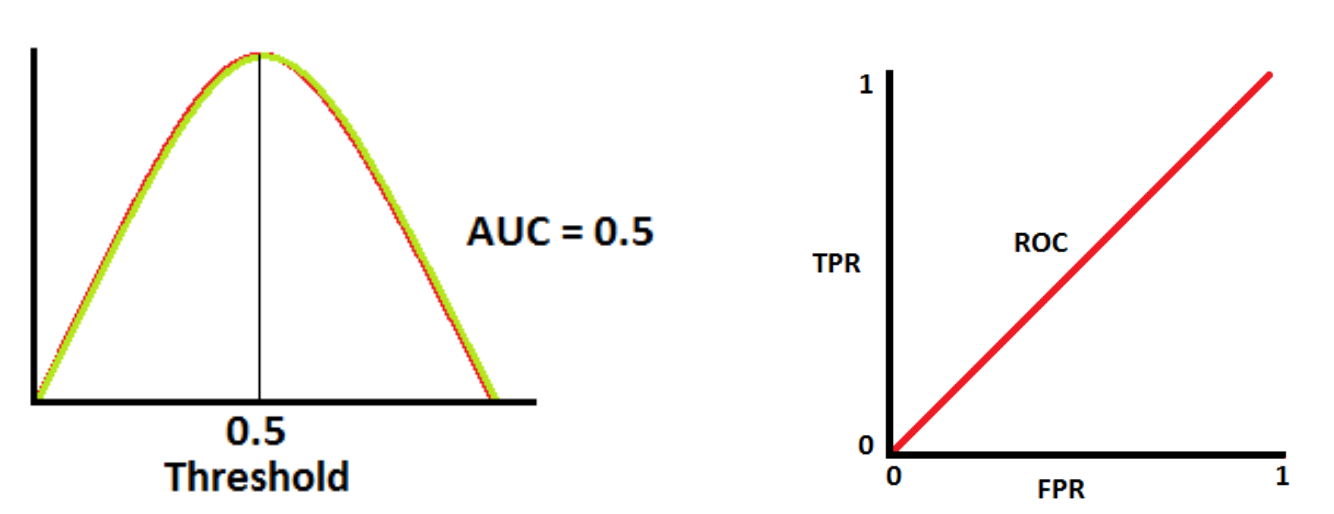
\includegraphics[scale=0.5]{AUC05.PNG}
\end{figure}
Cuando AUC es aproximadamente 0, el modelo en realidad está correspondiendo las clases. Significa que el modelo predice la clase negativa como una clase positiva y viceversa.
\begin{figure}[H]
\centering
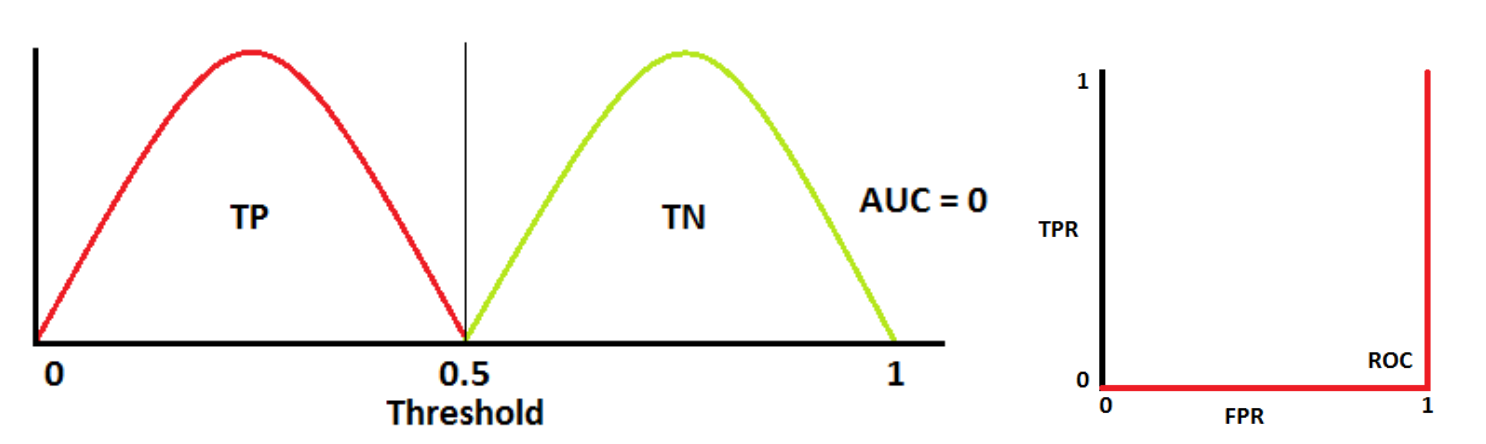
\includegraphics[scale=0.5]{AUC0.PNG}
\caption{AUC=0}
\end{figure}

\section{Desarrollo}
\subsection{Si se normaliza la base de datos que rendimiento tiene cada algortimo ?}
Para empezare a trabajar debemos preguntarnos lo siguiente:\\ ¿Para qué normalizar o reescalar variables?\\
Es necesario normalizar las variables ya que en la adquisición de datos estos pueden variar en valores muy altos o muy pequeños, formándose entre ellos unas brechas significativas, por lo cual una solución es ajustar los valores mediante la  normalizarlos o reescalar entre  (0,1).\\
A continuación, ser muestra los valores obtenidos mediante el uso de los algoritmos knn y bayesiano usando la base de datos sin normalizar.
\begin{multicols}{2}
\begin{figure}[H]
\centering
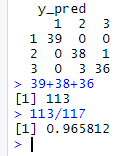
\includegraphics[scale=1]{knn.PNG}
\caption{Algoritmo K-nn}
\end{figure}
\begin{figure}[H]
\centering
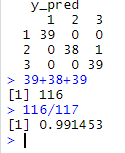
\includegraphics[scale=1]{bayesiano.PNG}
\caption{algoritmo Bayesiano}
\end{figure}
\end{multicols}
Donde se puede apreciar que poseen un rendimiento muy significativo, lo que nos indica que los algoritmos funcionan correctamente.\\
Otra forma de probar el rendimiento es reduciendo los valores de la base de datos, es decir reducir a una matriz con valores de calidad.\\
\begin{multicols}{2}
\begin{figure}[H]
\centering
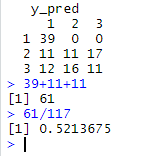
\includegraphics[scale=1]{knn con reduccion.PNG}
\caption{Algoritmo K-nn con matriz reducida}
\end{figure}
\begin{figure}[H]
\centering
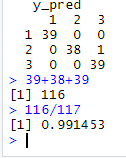
\includegraphics[scale=1]{bayes con reducucin.PNG}
\caption{Algoritmo bayesiano con matriz reducida}
\end{figure}
\end{multicols}
Donde se puede apreciar que el rendimiento del algoritmo K-nn cae significativamente ya que posee pocos vecinos, por otro lado el bayesiano mantiene su rendimiento.\\

A continuación, ser muestra los valores obtenidos mediante el uso de los algoritmos knn y bayesiano usando la base de datos normalizada.
\begin{multicols}{2}
\begin{figure}[H]
\centering
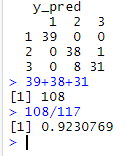
\includegraphics[scale=1]{knn_nor.PNG}
\caption{K-nn normalizado}
\end{figure}
\begin{figure}[H]
\centering
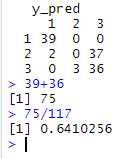
\includegraphics[scale=1]{bayes_norm.PNG}
\caption{Bayesiano normalizado}
\end{figure}
\begin{figure}[H]
\centering
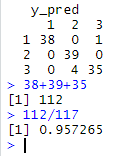
\includegraphics[scale=1]{knn_nor_con reduccion.PNG}
\caption{K-nn con matriz reducida y normalizada}
\end{figure}
\begin{figure}[H]
\centering
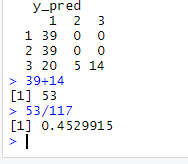
\includegraphics[scale=1]{bayes con reducucin_normT.PNG}
\caption{bayesiano con matriz reducida y normalizado}
\end{figure}
\end{multicols}

Con los datos normalizados existe una mejor en el algoritmo K-nn, donde se mantiene un buen rendimiento. El Bayesiano se reduce significativamente lo cual demuestra que dependiendo de el algoritmo es el rendimiento del modelo. 
\subsection{¿Funciona la selección de prototipos?}
El uso de prototipos proporciona un entrenamiento al momento de tratar los datos, enfocado al rendimiento que se determina al usar varios algoritmos, los cuales proporcionan los resultados de si la base de datos posee valores útiles.  
\subsection{Porcentualmente que variable aporta mayor datos al clasificador?}
Para el cálculo de las features selection se debe primeramente normalizar la base de datos .Para saber cuál variable aporta un mayor peso en la base de datos se utiliza el paquete boruta ,este paquete devuelve los porcentajes que aportan todas las variables de una base de datos basándose en un factor que en este caso será la etiqueta. La estructura de la función se muestra en la imagen posterior.
\begin{figure}[H]
\centering
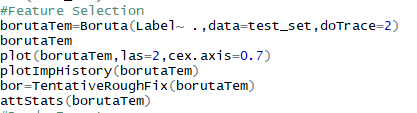
\includegraphics[scale=0.85]{curva.png}
\caption{Codígo en R para el desarrollo de porcentaje de datos}
\label{esquematic}
\end{figure}
Las variables existentes en la base de datos  son 4 ,de acuerdo a los resultados obtenidos ninguna de ellas tiene un peso lo suficientemente bajo para ser eliminada.Los valores a elimiar en este tipo de gráfica deben tener un color rojo ,los valores dudativos un color amarillo y los valores verdes con valores que son importantes para el modelo.
 Los porcentajes actuales de acuerdo al análisis realizado son :\\
\begin{itemize}
\item PH : 30/100
\item TDS: 25/100
\item Temperatura:20/100
\item Turbidez:15/100
\item Valores Sombra:10/100
\end{itemize}
\begin{figure}[H]
\centering
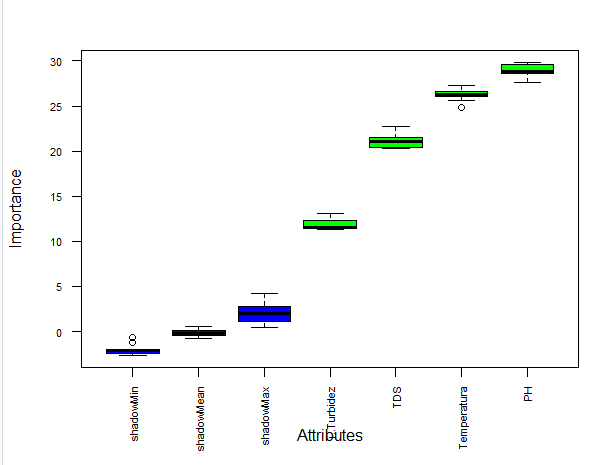
\includegraphics[scale=0.8]{graf.png}
\caption{Gráfica obtenida del porcentaje de variables dentro de la base de datos }
\label{esquematic}
\end{figure}

\subsection{Si se elimina la variable de menor importancia qué sucede con el clasificador?}
Después de haber obtenido los porcentajes de importancia de cada sensor y determinar que el sensor de Turbidez es el que tiene menor relevancia en la clasificación de los datos, vamos a realizar una prueba del clasificador KNN excluyendo los valores de dicho sensor.\\
Esto lo realizamos seleccionando las filas utilizadas en el algoritmo, cambiando los corchetes [,-5] por [,2:4], indicando que se tomaran las columnas de la 2 a la 4 como se aprecia en la Figura ~\ref{sin}.

\begin{figure}[H]
\centering
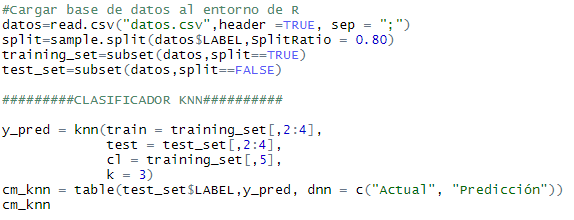
\includegraphics[scale=0.8]{sinTurb.png}
\caption{Código utilizado para aplicar KNN sin valores de turbidez}
\label{sin}
\end{figure}

Como resultados obtenemos que el utilizar o no los valores proporcionados por el sensor de turbidez no hace ninguna diferencia, los resultados obtenidos son exactamente los mismos en ambos casos (Figura ~\ref{res}). Esto quiere decir que es un sensor que bien puede retirarse de nuestro sistema y no influirá en los datos resultantes.

\begin{figure}[H]
\centering
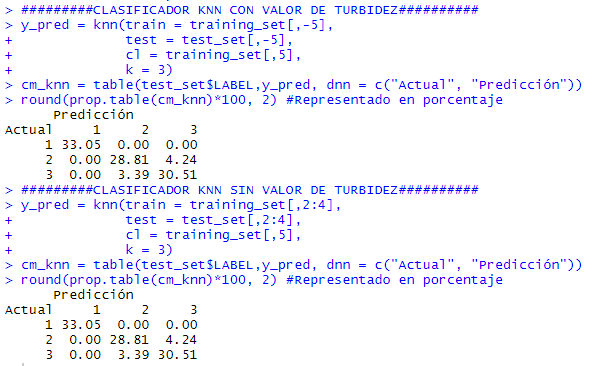
\includegraphics[scale=0.8]{res.png}
\caption{Resultados obtenidos con y sin sensor de Turbidez}
\label{res}
\end{figure}

\section{Conclusiones y Recomendaciones}

\subsection*{Conclusiones}
\begin{itemize}
\item El rendimiento de los diferentes algoritmos si se ve afectada si los valores están normalizados especialmente en el algoritmo bayesiano que de 99 por ciento baja a un pendiente del 55 por ciento, lo que permite saber que algoritmo es mejor.
\item Según el análisis realizado es bastante difícil la eliminación de algunos datos de la base de datos ,dado que todos presentan un nivel de porcentaje considerable además de que ninguno es representativo por sí mismo.
\item Uno de los resultados ha sido que el sensor de Turbidez no afecta en el comportamiento del clasificador, a partir del 15\% de importancia obtenido para este sensor podemos concluir que cualquier tasa de muestras extra con un porcentaje de importancia menor al 15\% no tendrá relevancia en nuestro sistema.
\end{itemize}

\subsection*{Recomendaciones}
\begin{itemize}
\renewcommand{\labelitemi}{$*$}
\item Una buena opción es la de remplazar los datos normalizados en la misma matriz para evitar crear nuevas variables que puedan producir errores debido a una mala interpretación de variables.
\item Los algoritmos de clasificación tienden a fallar cuando en la base de datos existe un cambio abrupto de valores, esto puede suceder al haber errores de lectura, por este motivo se recomienda asegurarse de tomar buenas lecturas y, a mayores realizar una revisión de la base de datos y corregir en caso de haber un error.
\end{itemize}

\bibliographystyle{ieeetran}%estilo referencia
\bibliography{Referencias}%archivo.bib
\end{document}